% !Mode:: "TeX:UTF-8"
% !TEX program  = xelatex
\documentclass[a4paper]{article}
\usepackage{amsmath}
\usepackage{amssymb}
\usepackage{ctex}
%\usepackage{braket}
%\usepackage[european]{circuitikz}
%\usepackage{hyperref}
%\hypersetup{pdfborder=0 0 0,pdfauthor="Yang Xu"}
\usepackage{multirow}
\usepackage{float}
\usepackage{graphicx}
\usepackage{url}
\usepackage{geometry}
\geometry{left=2.5cm,right=2.5cm,bottom=2.5cm,top=2.5cm}
\title{近代物理实验报告1.3:$\gamma$射线的吸收}
\author{xy\quad 学号\quad 匡亚明学院}
\date{2019年2月29日}
\begin{document}
\maketitle
\bibliographystyle{unsrt}
%--------main-body------------

\section{引言}
$\gamma$射线在穿透物质时,会被物质吸收,吸收作用的大小用吸收系数来表示。物质的吸收系数的值与$\gamma$射线的能量有关,也与物质本身的性质有关。正确测定物质的吸收系数,在核技术的应用与辐射防护设计中具有十分重要的意义。例如工业上广泛应用的料位计、密度计、厚度计,医学上的$\gamma$照相技术等都是根据这一原理研究设计的。

\section{实验目的}
\begin{enumerate}
    \item 了解$\gamma$射线在物质中的吸收规律。
    \item 掌握测量$\gamma$吸收系数的基本方法。
\end{enumerate}

\section{实验仪器}
$\gamma$源、单道分析器等。

\section{实验原理}

\subsection{窄束$\gamma$射线在物质中的吸收规律}
射线在穿过物质时,会与物质发生多种作用,主要有光电效应,康普顿效应和电子对效应,作用的结果使$\gamma$射线的强度减弱。

准直成平行束的$\gamma$射线称为窄束$\gamma$射线,单能窄束$\gamma$射线在穿过物质时,其强度的减弱服从指数衰减规律,即:
\begin{equation}
    I_x = I_0e^{-\mu x}\label{eq1}
\end{equation}

其中$I_0$为入射$\gamma$射线强度,$I_x$为透射$\gamma$射线强度,$x$为$\gamma$射线穿透的样品厚度,$\mu$为线性吸收系数。用实验的方法测得透射率$T = I_x/I_0$与厚度$x$的关系曲线,便可根据(\ref{eq1})式求得线性吸收系数$\mu$值。

为了减小测量误差,提高测量结果精度,实验上常先测得多组$I_x$与$x$的值,再用曲线拟合来求解。即:
\begin{equation}
    \ln(I_x) = \ln(I_0) - \mu x\label{eq2}
\end{equation}

由于$\gamma$射线与物质主要发生三种相互作用,三种相互作用对线性吸收系数$\mu$都有贡献,可得:
\begin{equation}
    \mu = \mu_{ph} + \mu_{c} + \mu_{p}\label{eq3}
\end{equation}
式中$\mu_{ph}$为光电效应的贡献,$\mu_{c}$为康普顿效应的贡献,$\mu_{p}$为电子对效应的贡献。它们的值不但与$\gamma$光子的能量$E_{\gamma}$有关,而且还与材料的原子序数、原子密度或分子密度有关。对于能量相同的$\gamma$射线不同的材料、$\mu$也有不同的值。图(\ref{fig1})表示铅、锡、铜、铝材料对$\gamma$射线的线性吸收系数$\mu$随能量$E_{\gamma}$变化关系。
\begin{figure}[!h]
    \centering
    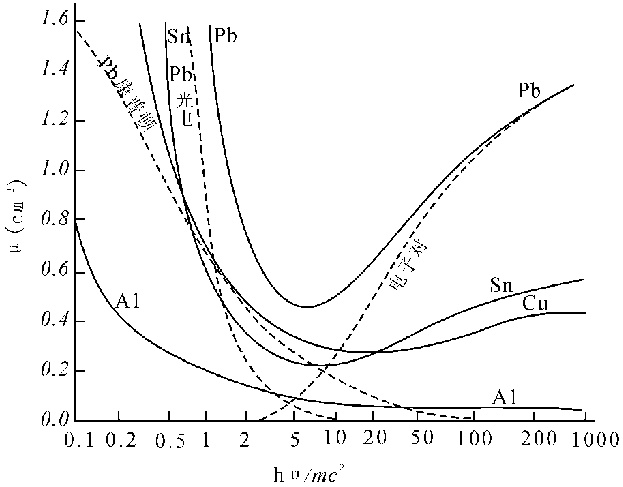
\includegraphics[width=0.6\textwidth]{fig/fig1.pdf}
    \caption{Pb、Sn、Cu、Al对$\gamma$射线的吸收系数和能量的关系}\label{fig1}
\end{figure}

图中横座标以$\gamma$光子的能量$h\nu$与电子静止能量$m_ec^2$的比值为单位,由图可见,对于铅低能$\gamma$射线只有光电效应和康普顿效应,对高能$\gamma$射线,以电子对效应为主。

为了使用上的方便,定义$\mu_m = \mu/\rho$为质量吸收系数,$\rho$为材料的质量密度。则(\ref{eq1})式可改写成如下的形式:
\begin{equation}
    I_x = I_0e^{-\mu_m x_m}\label{eq4}
\end{equation}
式中$x_m = x\rho$称为质量厚度,单位是$g/cm^2$。
\begin{figure}[!h]
    \centering
    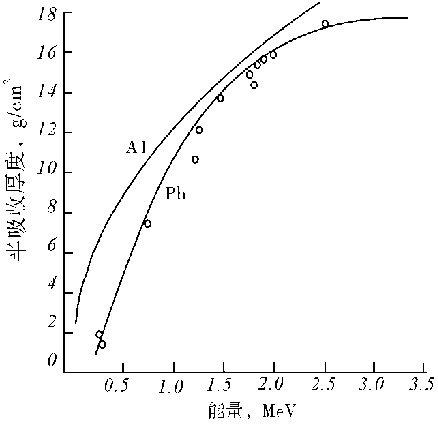
\includegraphics[width=0.4\textwidth]{fig/fig3.pdf}
    \caption{半吸收厚度和$\gamma$射线能量的关系}\label{fig3}
\end{figure}

\subsection{半吸收厚度}
物质对$\gamma$射线的吸收能力也常用半吸收厚度来表示,其定义为使入射$\gamma$射线强度减弱到一半所需要吸收物质的厚度。由(\ref{eq1})式可得
\begin{equation}
    x_{\frac12} = \frac{\ln2}{\mu}\label{eq5}
\end{equation}

显然,半吸收厚度$x_{\frac12}$与材料的性质和$\gamma$射线的能量都有关。图(\ref{fig3})表示铝、铅的半吸收厚度与$E_{\gamma}$的关系。若用实验方法测得$I_x$与$x$的变化关系,则可根据(\ref{eq3})式求得材料的线性吸收系数$\mu$值,从而由(\ref{eq5})式求得$x_{\frac12}$。

测量装置如图(\ref{fig2})所示。
\begin{figure}[!h]
    \centering
    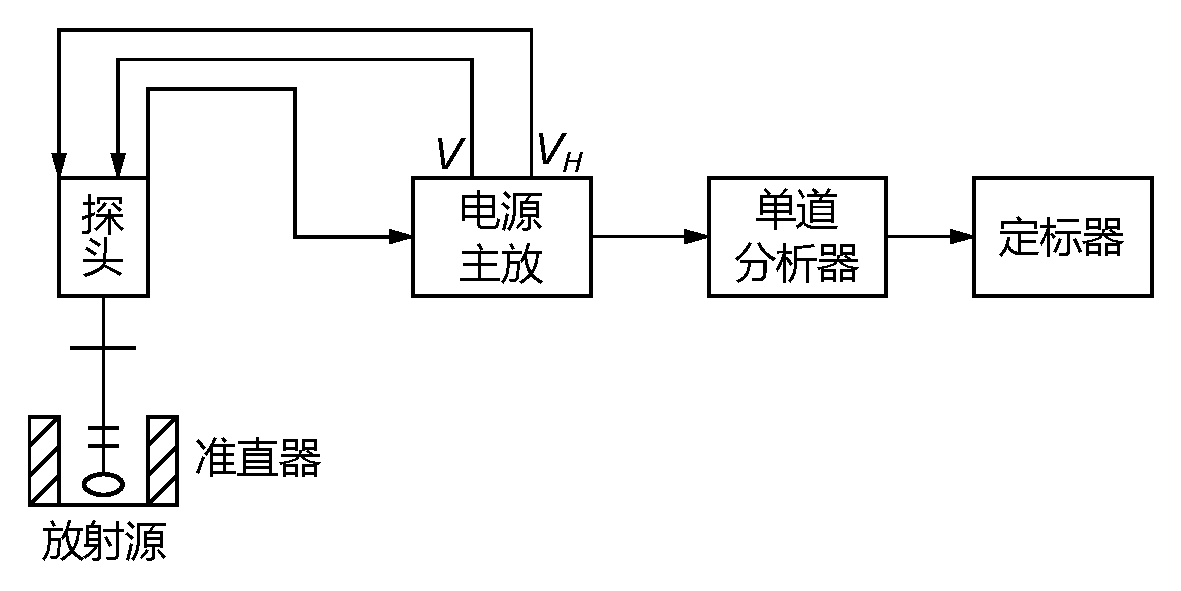
\includegraphics[width=0.8\textwidth]{fig/fig2.pdf}
    \caption{测量装置}\label{fig2}
\end{figure}

\section{实验内容}
\begin{enumerate}
    \item 按图(\ref{fig2})检查测量装置,调整探测器位置,使放射源、准直孔、探测器具有同一条水平线上。
    \item 打开系统电源,预热适当时间。
    \item 选择合适的高压值,放大倍数,和计数时间并保持不变。
    \item 测量不同吸收片厚度$x$时的计数$I_x$。
    \item 取出放射源,在相同条件下,测量本底计数$I_b$。
    \item 把高压降至最低值,关断电源。
    \item 用最小二乘法求出$\gamma$吸收系数$\mu$及半吸收厚度$d_{\frac12}$。
\end{enumerate}

\section{注意事项}
测量前必须认真阅读BH1224微机多道$\gamma$谱仪使用说明书。

\section{实验数据}
\subsection{数据}
所用$^{137}$Cs放射源编号:26;

强度:$S = 66.6\times 10^3\text{Bq}$;

能量:$E_r = 0.66\text{MeV}$;

计数时间:60s。

下列数据均为平均值。本底计数$I_B = 3563$。%;仅有放射源无样品时计数$I_0 = 9624$。

\subsubsection{Pb样品}
\begin{table}[!h]
\centering
\begin{tabular}{|c|c|c|c|c|c|}
\hline
编号	&	1	&	1+2	&	1+2+3	&	1+2+3+4	&	1+2+3+4+5 \\ \hline
厚度$x$/mm	&	2.07	&	4.79	&	6.75	&	9.21	&	11.34 \\ \hline
平均计数$I_x$/次	&	6864	&	6208	&	5700	&	5235	&	4833 \\ \hline
减去本底的计数$I_x$/mm & 3301 & 2645 & 2137 & 1672 & 1270\\ \hline
\end{tabular}
\caption{Pb的实验数据}\label{data:Pb}
\end{table}
\subsubsection{Cu样品}
\begin{table}[!h]
\centering
\begin{tabular}{|c|c|c|c|c|c|}
\hline
编号	&	1	&	2	&	3	&	4	&	1+4\\ \hline
厚度$x$/mm	&	10.08	&	14.56	&	20	&	24.2	&	34.42\\ \hline
平均计数$I_x$/次	&	7774	&	5505	&	5075	&	4622	&	4038\\ \hline
减去本底的计数$I_x$/mm & 4211 & 1942 & 1512 & 1059 & 475\\ \hline
\end{tabular}
\caption{Cu的实验数据}\label{data:Cu}
\end{table}
\subsubsection{Al样品}
\begin{table}[!h]
\centering
\begin{tabular}{|c|c|c|c|c|c|}
\hline
编号	&	1	&	2	&	3	&	4	&	1+4\\ \hline
厚度$x$/mm	&	10.3	&	14.8	&	19.58	&	24.58	&	34.9\\ \hline
平均计数$I_x$/次	&	7008	&	6922	&	6652	&	6448	&	5918\\ \hline
减去本底的计数$I_x$/mm & 3445 & 3359 & 3089 & 2885 & 2355\\ \hline
\end{tabular}
\caption{Al的实验数据}\label{data:Al}
\end{table}

\subsection{处理}
将表(\ref{data:Pb})$\sim$(\ref{data:Al})中的厚度$x$作为横坐标,减去本底的计数$I_x$的自然对数作为纵坐标,画图,并用最小二乘法进行线性拟合,求出拟合系数,如图(\ref{datafig})所示:
\begin{figure}[!h]
\centering
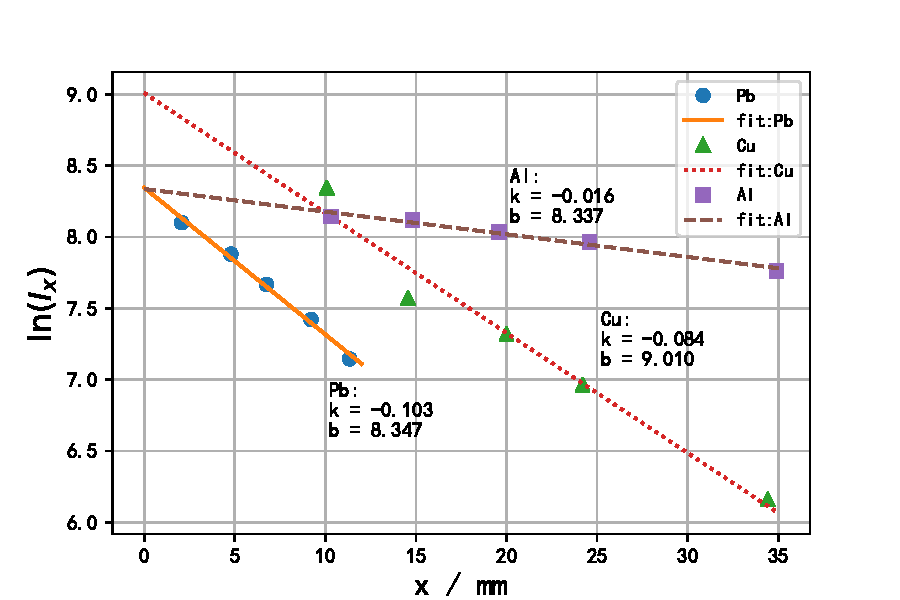
\includegraphics[width=\textwidth]{fig/all.pdf}
\caption{数据及拟合曲线}\label{datafig}
\end{figure}

从图(\ref{datafig})中可以得出各样品的$\gamma$吸收系数和半吸收厚度$d_{\frac{1}{2}}$,罗列如下:
\begin{enumerate}
\item $\mu_{\text{Pb}} = 0.103\text{mm}^{-1} = 1.03\text{cm}^{-1}$;$d_{\frac12}(\text{Pb}) = 6.74\text{mm}$。
\item $\mu_{\text{Cu}} = 0.084\text{mm}^{-1} = 0.84\text{cm}^{-1}$;$d_{\frac12}(\text{Cu}) = 8.24\text{mm}$。
\item $\mu_{\text{Al}} = 0.016\text{mm}^{-1} = 0.16\text{cm}^{-1}$;$d_{\frac12}(\text{Al}) = 43.67\text{mm}$。
\end{enumerate}

作为参考,查阅网络资料$^{\cite{ua}}$得知3种材料对$^{137}$Cs的660keV的$\gamma$光子的吸收系数(及计算得到的半吸收厚度)的文献值分别为:
\begin{enumerate}
\item $\mu_{\text{Pb}} = 1.19\text{cm}^{-1}$;$d_{\frac12}(\text{Pb}) = 5.82\text{mm}$。
\item $\mu_{\text{Cu}} = 0.94\text{cm}^{-1}$;$d_{\frac12}(\text{Cu}) = 7.37\text{mm}$。
\item $\mu_{\text{Al}} = 0.28\text{cm}^{-1}$;$d_{\frac12}(\text{Al}) = 24.76\text{mm}$。
\end{enumerate}

\section{误差分析}
\iffalse
对比文献值和测量值,我们发现铅和铜的数据较为符合,但是铝的实验结果偏差较大。

而实验过程中我们也观察到铝的测量数据不稳定的现象,有时加了辐射源的计数结果甚至比本底计数还低,因此测量了相当多次,取平均值。对于这一异常现象,我们暂时没有很好的解释。
\fi

\section{思考题}
\subsection{设铅的$\mu = 1.0\text{/cm}$,铝的$\mu = 0.2\text{/cm}$,为了使$\gamma$辐射强度将为原来的$1/10$,所需防护层厚度各为多少厘米?}
\subsection{待测的$\gamma$光子的能量与入射光子的能量是否相同?为什么?}
\subsection{实验布置中,为什么要把放射源、准直孔、探测器的中心保持在同一直线上?}
\subsection{何为半吸收厚度?其值与哪些因素有关?}
\subsection{为何铜、铝的吸收系数测量结果误差较大?}

\nocite{jiaocai}
\bibliography{ref}
\end{document}